\documentclass[12pt,a4paper]{scrreprt}
\usepackage[T1]{fontenc}
\usepackage[utf8]{inputenc}
\usepackage[ngerman]{babel}
%damit Tabellen direkt an der Stelle im Latex-Code auftauchen [H]
\usepackage{float}
%Zur Einbindung von Grafiken benötigt
\usepackage{graphicx}
%für Referenzen
\usepackage[backend=bibtex8, subentry]{biblatex}
%Verlinkungen für Inhaltsverzeichnis
\usepackage[colorlinks = true, linkcolor = black, citecolor = black, filecolor = black, urlcolor = black]{hyperref}
%Paket für Schriftarten
\usepackage{listings} 
\usepackage{csquotes}
\usepackage{scrhack}
%SQL-Schriftart
\lstset{language=Java,basicstyle=\footnotesize}

%bindet die source.bib ein
\bibliography{source}

%keine Einrückungen
%\setlength{\parindent}{0pt}

\begin{document}

% Titelblatt der Arbeit
  \begin{titlepage}

	\vspace*{0.5cm}

 \begin{center} \large 
    
    \huge {Universität Leipzig} \\
    \large Fakultät für Mathematik und Informatik \\
    Institut für Informatik \\
    \vspace*{2cm}

    {\huge Erstellen einer Webseite \\
    \vspace*{0.2cm}
    \huge für die Badminton-Domäne}
    \vspace*{1.5cm}

    Christoph Beger und Marcel Jacob \\ 
    \vspace*{0.5cm}
    angefertigt in der Abteilung Automatische Sprachverarbeitung
    \vspace*{1.5cm}

    Leipzig, den \today
    \vspace*{3cm}
    
  \end{center}
\end{titlepage} 
\newpage

%Inhaltsverzeichnis erstellen
\tableofcontents 

\chapter{Einleitung}
\section{Gegenstand und Motivation}
\subsection{Gegenstand}
Jede moderne, dynamische Website arbeitet mit einer oder mehreren Datenbanken als Datenbasis. Dadurch ist es leicht möglich die Webseiten flexibler und erweiterbar zu gestalten. Die Anzahl der Webseiten, die in reinem HTML-Code geschrieben sind, ist mittlerweile verschwindend gering geworden, da dies zu statisch ist. 

\subsection{Problematik}
Trotz der Fülle an vorhandenen Datenbanken im Netz, ist nur ein Bruchteil davon offen zugänglich. Dies kann beispielsweise aus Datenschutzgründen geschehen, um die privaten Informationen von Kunden vor fremden Zugriffen zu bewahren, oder aus Profitgründen, wenn ein Unternehmen mit den vorhandenen Daten Geld verdient. 

Die Daten sind also schlecht zugänglich und daher nicht für Analysezwecke geeignet. Außerdem besteht nicht die Möglichkeit Daten aus verschiedenen Quellen für eine Analyse zu vereinigen. 

\subsection{Motivation}
Da man aber beispielsweise über das Web-Interface viele Daten abgreifen kann, ist es möglich die vorhandenen Informationen aufzubereiten und eine eigene Datenbank für diese zu erstellen. Dieses Szenario lässt sich auf eine Vielzahl von Domänen anwenden. In dieser Arbeit liegt der Fokus auf einer speziellen Domäne: Badminton. Wie auch in anderen Sportarten, gibt es eine Weltrangliste für Teams oder einzelne Spieler, die von einer Organisation verwaltet und regelmäßig aktualisiert wird. Für die Rangliste beim Badminton ist die Badminton World Federation (BWF) zuständig, welche über folgenden Link erreicht werden kann: http://bwf.tournamentsoftware.com/home.aspx \cite{BWF2015}

\section{Zielsetzung}
Ziel der Arbeit soll es sein, die entsprechenden HTML-Dokumente für die einzelnen Spieler herunterzuladen, aus diesen die relevanten Daten zu extrahieren und in eine eigenkonzipierte Datenbank zu importieren, um im Anschluss ein Webfrontend für eine angemessene Repräsentation und Zugänglichkeit der Informationen zu erstellen.
\chapter{Grundlagen}
\section{Django}
\label{Django}
Django ist ein Framework, mit dessen Hilfe Webseiten erstellt werden können. Dafür setzt Django auf die Programmiersprache Python und legt Wert auf Wiederverwendbarkeit der einzelnen Komponenten. Es folgt einem Model-Template-View Muster, welches sich an dem Model-View-Controller Schema orientiert. Mit Hilfe eines Objekt-relationalen Mappers (ORM) werden die geschriebenen Models in Datenbankstrukturen überführt und die Anfragen ausgeführt. Zum Testen der erstellten Webseite bringt Django einen Entwicklungs-Webserver mit. Django wird derzeit aktiv entwickelt, die neueste Version ist die 1.8 (Stand 06. April 2015).

\section{PostgreSQL}
Als Daten haltendes Backend haben wir das objektrelationale Datenbankmanagementsystem (DBMS) PostgreSQL \cite{PostgreSQL2015} ausgewählt. Das DBMS ist open-source und unterstützt einen Großteil des SQL-Standards. Zudem lässt sich PostgreSQL um eine Vielzahl von eigenentwickelten Komponenten erweitern.\\

\noindent Beispielsweise können folgende Komponenten selbst definiert werden:
\begin{itemize}
\item Datentypen
\item Funktionen
\item Operatoren 
\item u.v.m.
\end{itemize}
\chapter{Vorüberlegungen}
\section{Crawling und Parsing relevanter Webseiten}
Zunächst mussten die relevanten Webseiten identifiziert werden. Die größte und bekannteste Webseite, für welche wir uns auch als Grundlage für unsere Datenbasis entschieden haben, ist die Seite der Badminton World Federation (BWF) \cite{BWF2015}. Diese enthält sowohl Informationen über die derzeit aktiven Spieler, als auch Ergebnisse zu internationalen Turnieren, wobei für uns die Extraktion der Spielerinformationen Priorität haben sollte. \newline \newline
Wir sind bei der Analyse der Webseitenstruktur zu der Erkenntnis gekommen, dass alle, für unsere Datensammlung nötigen Informationen in den  "`biography.aspx"' Seiten hinterlegt sind. Diese Seiten besitzen alle eine Spieler-ID, die in der URL als GET-Parameter übergeben wird. Daraus ergeben sich zwei Möglichkeiten der Herangehensweise. 
\begin{enumerate}
\item Gezieltes lokalisieren der Profilseiten
\item Finden aller Spieler-IDs, um sie anschließend für das Abrufen der "`biography.aspx"'- Seiten zu nutzen
\end{enumerate}
Dabei setzen beide Möglichkeiten an einem Crawling der "`ranking.aspx"'-Seiten an, wo zu jeder Spielgruppe (Men's Singles, Women's Singles, Men's Doubles, Women's Doubles, Mixed Doubles) alle Spieler, sortiert nach Platzierung in der jeweiligen Gruppe, gelistet sind.

\subsection{Aufbau der Profilseite}

Die Profilseite gliedert sich in zwei Abschnitte (siehe Abbildung \ref{fig:bwf_profile}). Der obere Abschnitt beinhaltet allgemeine Informationen über den Spieler, wie zum Beispiel Namen und Geburtsdatum. \newline

Im unteren Abschnitt sind weiterführende Informationen enthalten, die sich auf die beiden Bereiche "`Biodata"' und "`Athlete Profile"' aufteilen. Interessant für unsere Datensammlung ist dort vor allem der erstgenannte Bereich, da die darin enthaltenen Daten besser über alle Spieler verglichen werden können. Beispielsweise findet man im ersten Bereich die Größenangabe und den Geburtsort.

\begin{figure}[H]
\centering
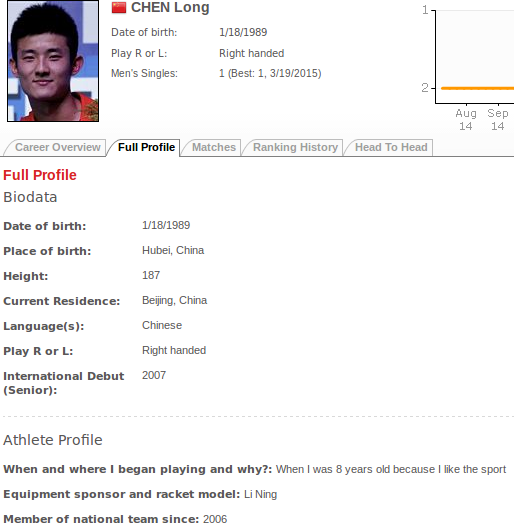
\includegraphics[scale=0.4]{images/bwf_profile}
\caption{Ausschnitt aus der Profilseite der BWF-Webseite}
\label{fig:bwf_profile}
\end{figure}

\section{Gestaltung des Frontends}
Für die Gestaltung des Frontends haben wir uns folgende, mögliche Strukturierung überlegt:\\

\noindent\textbf{Search-Seite mit einer Liste aller Spieler:}
\begin{itemize}
\item Die Seite soll aus zwei Teilen bestehen. Der obere Teil dient zur Spezifizierung von Suchkriterien, während der untere Teil die Ergebnismenge in Form einer Tabelle darstellen soll.
\item Die Filter- und Suchfunktion des oberen Teils der Seite wird mit einem Formular realisiert, in dem zu allen Attributen einer Person Werte spezifiziert werden können. Neben der exakten Suche sollen die Felder auch ähnliche Werte finden (z.B. Eingabe des Nachnamens "`Berg"' liefert Treffer mit Nachnamen "`Berg"' und "`Bergmann"'). Die Eingabefelder sollen den Datentypen der Attribute entsprechend angepasst sein, durch zum Beispiel Textfelder, Auswahllisten, usw.
\item Paging (Auswahlmöglichkeit wie viele Spieler pro Seite angezeigt werden sollen)
\item Das Suchergebnis soll nach Spalten sortierbar sein, sowohl auf-, als auch absteigend.
\item Optional: Benutzer kann die anzuzeigenden Tabellenspalten selber wählen.
\end{itemize}

\noindent\textbf{Detail-Seite für ausgewählten Spieler:}
\begin{itemize}
\item Darstellung aller Informationen zu einem Spieler
\item Anzeige des Profilbildes
\item Attributwerte, die sich aus externen Tabellen ergeben (z.B. club oder nationality) sollen als Hyperlink auf die Search-Seite angezeigt werden, wo alle Spieler mit dem jeweiligen Attribut aufgelistet werden.
\item Wenn Attributwerte nicht gesetzt sind, sollen diese noch nachträglich eintragbar sein. Dazu muss es einen Verweis von dieser Seite auf eine Edit-Seite geben.
\item Optional: Grafik zum Rankingverlauf
\end{itemize}

\noindent\textbf{Profilbearbeitung:}
\begin{itemize}
\item Die Seite sollte nur durch einen Redirect von einer Detail-Seite eines Spielers erreichbar sein.
\item In einem Formular sollen alle Attribute eines Spielers angezeigt werden, die noch nicht gesetzt sind.
\item Nach einem Submit werden die Werte in der Datenbank nachgetragen und man wird zurück zur Detail-Seite verwiesen.
\end{itemize}

\noindent\textbf{Query-Seite zum Erstellen von Abfragen:}
\begin{itemize}
\item Auf dieser Seite wird es ein Freitextfeld geben, wo der Nutzer eigene SQL-Anfragen eintragen kann.
\item Es dürfen nur SELECT-Anfragen ausgeführt werden.
\item Das Ergebnis der Anfrage wird unter dem Freitextfeld in Form einer Tabelle angezeigt.
\end{itemize}

\noindent\textbf{Seite für die grafische Darstellung}
\begin{itemize}
\item Fokussierung auf Häufigkeitsanalysen, da die benutzer-spezifischen Auswertungen zu komplex werden könnten und den Rahmen des Projekts sprengen würden.
\item Darstellungsart der Ergebnisse sollte der Problematik angepasst sein. (Histogramm, Kuchendiagramm, Balkendiagramm) 
\end{itemize}
\chapter{Umsetzung}
\section{Systemvoraussetzungen}
Python, Django-Installation, Pakete (Versionen...)

\section{Aufbau des Backend}
\label{Backend}
Zunächst musste ein Crawler geschrieben werden, der die entsprechenden Webseiten herunterlädt und abspeichert. Diesen Schritt haben wir mit Hilfe von Java umgesetzt. 

Da es den Anschein hatte, dass der Server den Zugriff nach ca. 100 Dokumenten verweigert, wurde der Crawler um eine Funktion erweitert, mit deren Hilfe man einen Webproxy zwischenschalten kann, der dieses Problem löst. Sobald ein Dokument nicht heruntergeladen werden kann, wird der nächste Proxy aus der Liste genommen. Die Proxy-Liste stammt von http://proxylist.hidemyass.com/ \cite{HMA2015}. Insgesamt wurden 7854 Dokumente heruntergeladen.\\

Im nächsten Schritt wurde ein Perl-Skript geschrieben, welches die vorhandenen Informationen extrahiert und in eine PostgreSQL Datenbank importiert. Hierfür wurde vorher ein entsprechendes Schema, welches in der folgenden Abbildung dargestellt ist, erstellt. Das Schema spiegelt die Informationen wider, die extrahiert und für den Import in die Datenbank normalisiert wurden. Hierzu zählen beispielsweise Informationen wie Geburtstag, Geburtsort, Größe und Links-/Rechtshänder.

\begin{figure}[H]
\centering
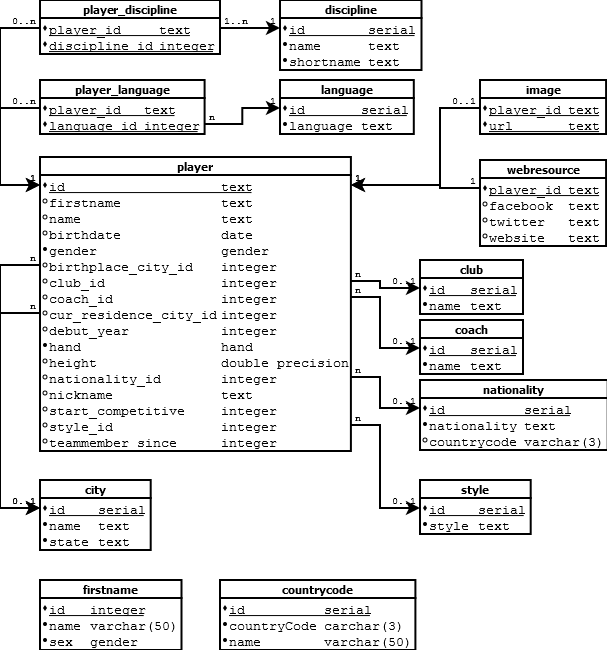
\includegraphics[width=1\textwidth]{images/ER-Diagramm} 
\caption{ER-Diagramm}
\label{fig:ER-Diagramm}
\end{figure}

\section{Aufbau des Frontend}
\label{Frontend}
Die erstellte Webseite soll gut lesbar, schnell zu laden und intuitiv zu bedienen sein. Dafür wurde auf der Startseite ein kleines Navigationsmenü zur Unterteilung der einzelnen Features eingerichtet. 

Auf der Startseite erhält man einen kleinen Begrüßungstext, der das Ziel und die Funktionen der Webseite kurz beschreibt. Mit dem Suchformular ist es möglich, nach Spielern zu suchen, die gewisse Bedingungen erfüllen. Klickt man auf die etwas längliche Spieler-Id, werden alle wichtigen Informationen und, wenn vorhanden ein Bild des Spielers, angezeigt. Hier ist es auch möglich bestimmte Informationen für den Spieler zu setzen, wenn diese noch "`NULL"' sind. Sucht man beispielsweise nach dem deutschen Badmintonspieler Marc Zwiebler, ist es nur möglich den Verein einzutragen, da alle anderen Werte bereits gesetzt sind und viele Werte wie Geburtstag, Name und Geschlecht sich im Laufe des Lebens nicht ändern.

Außerdem gibt es eine Reihe von vordefinierten Statistiken, die auf Basis der Datenbank erstellt wurden. Hierzu zählen:
Links- vs. Rechtshänder, Verein, Coach, Disziplin, Geschlecht, gesprochene Sprache/Muttersprache, aktuelle Nationalität und die Körpergröße. Zu guter Letzt gibt es einen Editor, mit dem Nutzer SQL-Anfragen schreiben können, um ihre eigenen Informationsbedürfnisse zu stillen.
\chapter{Erkenntnisse}
\label{Erkenntnisse}
Laut dem NTV-Artikel \cite{Hand2015}, wird der Anteil der Linkshänder in der Bevölkerung auf 10 bis 15\% geschätzt, ihr Anteil läge im Spitzensport in einigen Sportarten aber bei bis zu 55\%. Betrachtet man nun unsere mageren 8,81\% für den Anteil der Linkshänder, bekommt man den Eindruck, dass die Linkshänder im Nachteil wären. Eine kurze manuelle Auswertung der aktuellen Weltrangliste (Stand 18. Februar 2015) für das Herren- und das Dameneinzel für die ersten 25. Plätze, ergibt jedoch einen höheren Anteil der Linkshänder. Bei den Männern sind 6 der 25 Topleute Linkshänder, bei den Frauen sind es immerhin 4. Dies ergibt einen Anteil von 20\%, welcher immerhin etwas über dem Anteil an der Gesamtbevölkerung liegt und den vermeintlichen Nachteil in einen Vorteil wandelt. Dennoch sind die Daten mit Vorsicht zu genießen, da ebenfalls die Top-100 hätten ausgewertet werden können, was in der Folge wiederum zu anderen Zahl führt.

Für die Geschlechterverteilung ergibt sich ein geringes Ungleichgewicht zugunsten der Männer, die 59,8\% einnehmen. Bei der Länderverteilung belegt Indonesien mit 521 Spitzensportlern den ersten Platz, gefolgt von Großbritannien mit 363 Spielern. Deutschland belegt mit 199 Spielern den 9. Rang. Insgesamt lässt sich ein Trend in den asiatischen Ländern und in Europa erkennen, welche einen Großteil aller Spieler einnehmen.\\

Bei den Statistiken zu dem Verein, dem Coach, der gesprochenen Sprache und der Körpergröße lässt sich sagen, dass hier nur sehr wenige Daten vorhanden sind. Daher lässt sich keine allgemeine Aussage für diese Werte treffen.

\section{Fehler und Verbesserungsmöglichkeiten}
Der selbst geschriebene Crawler hält sich nicht an gängige Richtlinien, die ein "`richtiger"' Crawler einhalten würde. Beispielweise müsste man nach einer "`robots.txt"' suchen, damit man weiß welche Dokumente man crawlen darf und welche nicht. Außerdem müsste sich ein Crawler im HTTP-Protokoll über das Feld "`user-agent"' erkennbar machen, da es sich nicht um einen normalen Nutzer handelt. Um den Server nicht zu überlasten, müssten Wartezeiten eingehalten werden, bevor das nächste Dokument gecrawlt werden kann.\\

Im Bereich des Profil-Updates sind einige Verbesserungsmöglichkeiten denkbar. Man könnte beispielsweise ein Update für alle Werte erlauben, die sich im Laufe eines Lebens ändern können, auch wenn diese bereits gesetzt sind. Hierzu zählt auch der Nachname, der sich bei einer Heirat ändern kann. Für die Qualität der Datenbank wäre es wichtig, die geänderten Werte nicht einfach zu übernehmen, sondern als Vorschläge in einer gesonderten Tabelle abzuspeichern und manuell überprüfen zu lassen.\\

Verein, Coach als Text? Größe nur im Bereich 100-220 cm?

\section{Erweiterungsmöglichkeiten}
Es wäre denkbar die Webseite zu "`vervollständigen"', da in der Datenbank noch viele Informationen zu den Spielern leer sind. Dafür könnte man weitere Seiten crawlen und parsen, um die Lücken im Datenbestand zumindest teilweise zu schließen. Außerdem lassen sich weitere Informationen in die Webseite einpflegen. Beispielsweise könnten die Regeln für Badminton ergänzt oder interessante Matches zwischen den Top-Spielern als Video eingebettet werden. Selbstverständlich sind weitere Möglichkeiten für die Visualisierungen mit den vorhandenen Daten denkbar.

\chapter*{Zusammenfassung}
\addcontentsline{toc}{chapter}{Zusammenfassung}
Durch den Einsatz verschiedener Technologien und Werkzeuge ist es gelungen, aus schlecht zugänglichen Daten eine Webseite zu erstellen, die interessante Aspekte der Daten visualisieren kann. Im gesamten Prozess der Entwicklung ging es auch um das Kennenlernen neuer Technologien, vor allem im Bereich Webdesign.

\chapter*{Literaturverzeichnis}
\addcontentsline{toc}{chapter}{Literaturverzeichnis}
\printbibliography	

\end{document}